\documentclass[a4paper]{article}
\usepackage[a4paper, total={155mm, 250mm}]{geometry}
\usepackage{amssymb}
\usepackage[nodayofweek]{datetime}

\usepackage{wrapfig}
\usepackage{tikz}

\tikzset{
	r/.style={red!30},
	g/.style={green!30},
	b/.style={blue!30},
	ye/.style={yellow!40},
}

\newcommand{\half}{\frac{1}{2}}
\newcommand{\hexpr}[1]{\half(#1^2 + #1 + 2)}

\title{Splitting the Plane}
\author{Dyson}
\date{\today}

\begin{document}

\maketitle

\setlength{\parindent}{0em}
\setlength{\parskip}{1em}

Challenge question 3 of Review Exercise 2 in the Edexcel Further Maths Core Pure Book 1 says:\begin{center}Prove that if $n$ non-parallel lines divide the plane into $r$ regions, then $2n \leq r \leq \hexpr{n}$.\end{center}

I've also seen this problem presented as cutting pizza, and using circles looks nice, so I'll be doing that throughout.

\begin{figure}[h]
\centering
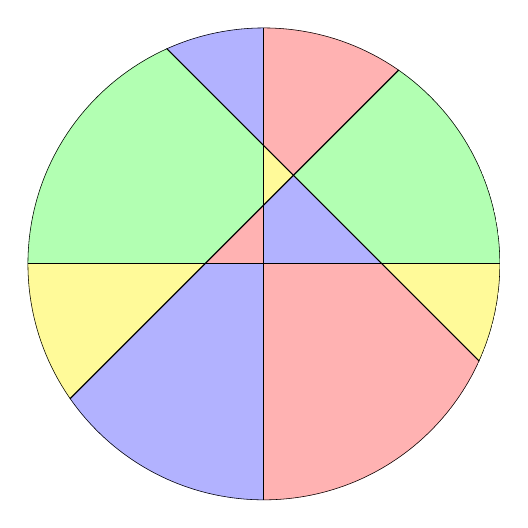
\begin{tikzpicture}[scale=3]
	\clip (0,0) circle[radius=1];

	\coordinate (A) at (0.125,0.375);

	\fill [r] (0,1) -- (0,0.5) -- (A) -- (0.75,1);
	\fill [g] (1,1) -- (0.75,1) -- (A) -- (0.5,0) -- (1,0);
	\fill [b] (A) -- (0,0.25) -- (0,0) -- (0.5,0);
	\fill [ye] (0,0.25) -- (0,0.5) -- (A);
	\fill [b] (0,1) -- (0,0.5) -- (-0.5,1);
	\fill [g] (-1,1) -- (-0.5,1) -- (0,0.5) -- (0,0.25) -- (-0.25,0) -- (-1,0);
	\fill [r] (0,0) -- (0,0.25) -- (-0.25,0);
	\fill [ye] (-0.25,0) -- (-1,-0.75) -- (-1,0);
	\fill [b] (0,0) -- (-0.25,0) -- (-1,-0.75) -- (-1,-1) -- (0,-1);
	\fill [r] (0,0) -- (0,-1) -- (1,-1) -- (1,-0.5) -- (0.5,0);
	\fill [ye] (0.5,0) -- (1,0) -- (1,-0.5);

	\draw (0,0) circle[radius=1];

	\draw (0,1) -- (0,-1);
	\draw (-1,0) -- (1,0);
	\draw (1,-0.5) -- (-0.5,1);
	\draw (-1,-0.75) -- (0.75,1);
\end{tikzpicture}
\hspace{10ex}
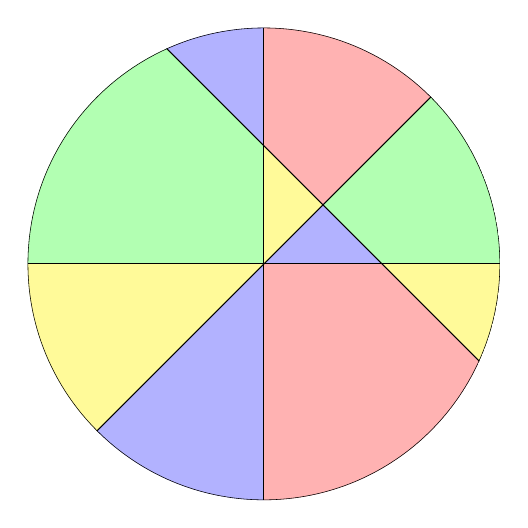
\begin{tikzpicture}[scale=3]
	\clip (0,0) circle[radius=1];

	\fill [r] (0,1) -- (0,0.5) -- (0.25,0.25) -- (1,1);
	\fill [g] (1,1) -- (0.25,0.25) -- (0.5,0) -- (1,0);
	\fill [b] (0.25,0.25) -- (0,0) -- (0.5,0);
	\fill [ye] (0,0) -- (0,0.5) -- (0.25,0.25);
	\fill [b] (0,1) -- (0,0.5) -- (-0.5,1);
	\fill [g] (-1,1) -- (-0.5,1) -- (0,0.5) -- (0,0) -- (-1,0);
	\fill [ye] (0,0) -- (-1,-1) -- (-1,0);
	\fill [b] (0,0) -- (-1,-1) -- (-1,-1) -- (0,-1);
	\fill [r] (0,0) -- (0,-1) -- (1,-1) -- (1,-0.5) -- (0.5,0);
	\fill [ye] (0.5,0) -- (1,0) -- (1,-0.5);

	\draw (0,0) circle[radius=1];

	\draw (0,1) -- (0,-1);
	\draw (-1,0) -- (1,0);
	\draw (1,-0.5) -- (-0.5,1);
	\draw (-1,-1) -- (1,1);
\end{tikzpicture}
\caption{An example of $n = 4$ with 11 regions (left) and 10 regions (right)}
\end{figure}

\section{Basis}

\begin{wrapfigure}[5]{l}{0.3\linewidth}
\vspace{-1em}
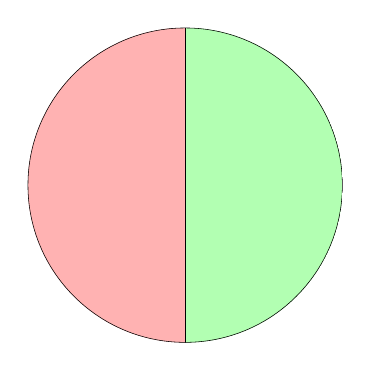
\begin{tikzpicture}[scale=2]
	\clip (0,0) circle[radius=1];

	\fill [r] (-1,1) rectangle (0,-1);
	\fill [g] (0,1) rectangle (1,-1);

	\draw (0,0) circle[radius=1];

	\draw (0,1) -- (0,-1);
\end{tikzpicture}
\end{wrapfigure}

For $n = 1$, we have one line, and we can only split the plane into 2 regions. This basis satisfies the inequality that we're looking for. For the minimum, $2n = 2 \times 1 = 2$ and for the maximum, $\hexpr{n} = \hexpr{1} = \half \times 4 = 2$. And of course, $2 \leq 2 \leq 2$, so the statement holds for $n = 1$.

\vspace{4em}

\section{Assumption}

We will now assume that if $k$ non-parallel lines cut the plane into $r$ regions, then $2k \leq r \leq \hexpr{k}$. We have shown this to be true for $k = 1$, so we can now use mathematical induction to show it to be true for any $k + 1$, and then we will have proved the original statement for all $n \in \mathbb{Z}^+$.

\newpage

\section{Induction}

We will start by showing the minimum number of regions for $k + 1$ lines. We are going to start with $k$ lines and add one more, so we start with $2k$ regions, as shown in the left circle here with $k = 3$.

Note that all the lines pass through a central point. This intersection point is shared by all the lines and is the only intersection point here. When we add our $(k + 1)$th line, we also want it to pass through this point to minimise how many new regions we create. When it does, it must cut through exactly two regions, turning two regions into four and giving us two new regions. Therefore, the minimum number of regions for $k + 1$ lines is $2k + 2 = 2(k + 1)$, as expected.

\begin{figure}[h]
\centering
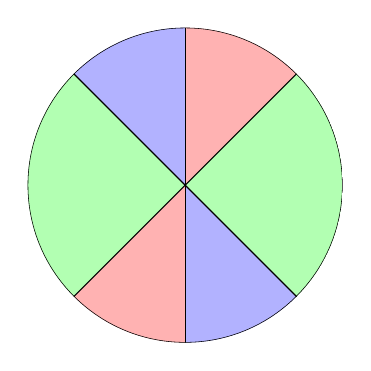
\begin{tikzpicture}[scale=2]
	\clip (0,0) circle[radius=1];

	\fill [r] (0,1) -- (0,0) -- (1,1);
	\fill [g] (1,1) -- (0,0) -- (1,-1);
	\fill [b] (1,-1) -- (0,0) -- (0,-1);
	\fill [r] (0,-1) -- (0,0) -- (-1,-1);
	\fill [g] (-1,-1) -- (0,0) -- (-1,1);
	\fill [b] (-1,1) -- (0,0) -- (0,1);

	\draw (0,0) circle[radius=1];

	\draw (0,1) -- (0,-1);
	\draw (-1,-1) -- (1,1);
	\draw (-1,1) -- (1,-1);
\end{tikzpicture}
\hspace{15ex}
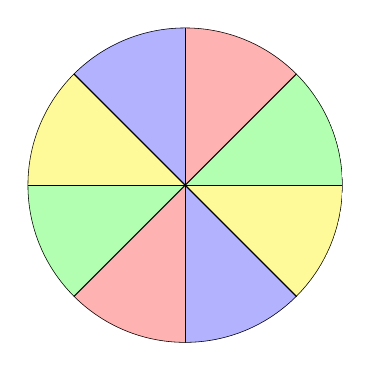
\begin{tikzpicture}[scale=2]
	\clip (0,0) circle[radius=1];

	\fill [r] (0,1) -- (0,0) -- (1,1);
	\fill [g] (1,1) -- (0,0) -- (1,0);
	\fill [ye] (1,0) -- (0,0) -- (1,-1);
	\fill [b] (1,-1) -- (0,0) -- (0,-1);
	\fill [r] (0,-1) -- (0,0) -- (-1,-1);
	\fill [g] (-1,-1) -- (0,0) -- (-1,0);
	\fill [ye] (-1,0) -- (0,0) -- (-1,1);
	\fill [b] (-1,1) -- (0,0) -- (0,1);

	\draw (0,0) circle[radius=1];

	\draw (0,1) -- (0,-1);
	\draw (-1,-1) -- (1,1);
	\draw (-1,1) -- (1,-1);
	\draw (-1,0) -- (1,0);
\end{tikzpicture}
\end{figure}

The maximum number of lines is a bit more complicated. All these lines are non-parallel by definition, which means that a $(k + 1)$th line will intersect all $k$ previous lines. If they all intersect at a single point, then we get the minimum number of regions, but if every intersection point is between only two lines, then we get the maximum number of regions.

When a new line intersects an existing one, it adds two new regions, as seen previously. When we add a $(k + 1)$th line, this is true for each of the $k$ previous lines, so we'd expect $2k$ new regions. However, $k - 1$ of these regions are double-counted, so we disregard them and get $k + 1$ new regions.

To understand this, consider the case of $k = 2$. We can start with two orthogonal lines and consider each separately. When we cut through the horizontal line shown here, we add 2 regions, one above the line and one below, shown in yellow and blue.

\begin{figure}[h]
\centering
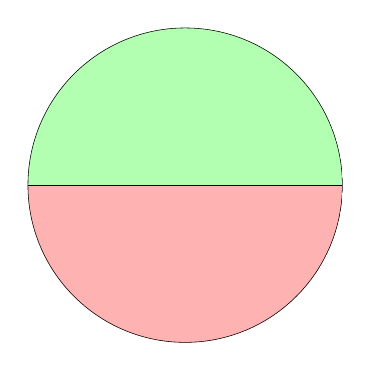
\begin{tikzpicture}[scale=2]
	\clip (0,0) circle[radius=1];

	\fill [r] (-1,0) rectangle (1,-1);
	\fill [g] (-1,0) rectangle (1,1);

	\draw (0,0) circle[radius=1];

	\draw (1,0) -- (-1,0);
\end{tikzpicture}
\hspace{15ex}
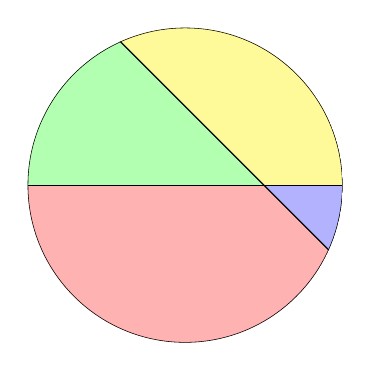
\begin{tikzpicture}[scale=2]
	\clip (0,0) circle[radius=1];

	\fill [r] (-1,-1) -- (-1,0) -- (0.5,0) -- (1,-0.5) -- (1,-1);
	\fill [g] (-1,1) -- (-1,0) -- (0.5,0) -- (-0.5,1);
	\fill [b] (1,0) -- (0.5,0) -- (1,-0.5);
	\fill [ye] (1,1) -- (1,0) -- (0.5,0) -- (-0.5,1);

	\draw (0,0) circle[radius=1];

	\draw (-1,0) -- (1,0);
	\draw (1,-0.5) -- (-0.5,1);
\end{tikzpicture}
\end{figure}

When we cut through the vertical line, we similarly get 2 new regions.

\begin{figure}[h]
\centering
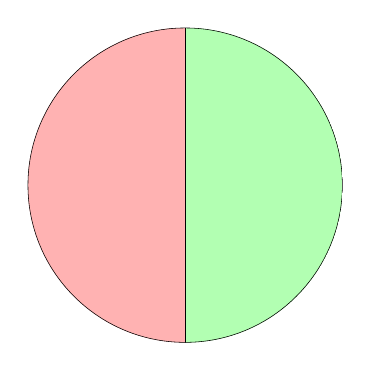
\begin{tikzpicture}[scale=2]
	\clip (0,0) circle[radius=1];

	\fill [r] (0,1) rectangle (-1,-1);
	\fill [g] (0,1) rectangle (1,-1);

	\draw (0,0) circle[radius=1];

	\draw (0,1) -- (0,-1);
\end{tikzpicture}
\hspace{15ex}
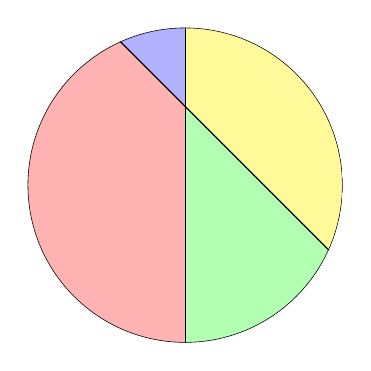
\begin{tikzpicture}[scale=2]
	\clip (0,0) circle[radius=1];

	\fill [r] (-1,1) -- (-1,-1) -- (0,-1) -- (0,0.5) -- (-0.5,1) -- (-1,1);
	\fill [g] (1,-1) -- (0,-1) -- (0,0.5) -- (1,-0.5);
	\fill [b] (0,1) -- (0,0.5) -- (-0.5,1);
	\fill [ye] (1,1) -- (0,1) -- (0,0.5) -- (1,-0.5);

	\draw (0,0) circle[radius=1];

	\draw (0,1) -- (0,-1);
	\draw (1,-0.5) -- (-0.5,1);
\end{tikzpicture}
\end{figure}

\newpage

So when we combine these two to create a diagram with 3 total lines, we could reasonably expect 8 total regions, but this isn't the case. We actually get 7, as shown. This is because we double-count one region when we combine the diagrams. In this case, we end up double-counting the resultant yellow region.

\begin{center}
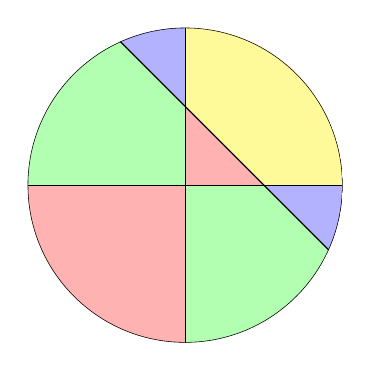
\begin{tikzpicture}[scale=2]
	\clip (0,0) circle[radius=1];

	\fill [r] (0,0) rectangle (-1,-1);
	\fill [ye] (1,1) -- (1,0) -- (0.5,0) -- (0,0.5) -- (0,1);
	\fill [r] (0,0) -- (0,0.5) -- (0.5,0);
	\fill [g] (0,-1) -- (0,0) -- (0.5,0) -- (1,-0.5) -- (1,-1);
	\fill [g] (-1,1) -- (-1,0) -- (0,0) -- (0,0.5) -- (-0.5,1);
	\fill [b] (1,0) -- (0.5,0) -- (1,-0.5);
	\fill [b] (0,1) -- (0,0.5) -- (-0.5,1);

	\draw (0,0) circle[radius=1];

	\draw (0,1) -- (0,-1);
	\draw (-1,0) -- (1,0);
	\draw (1,-0.5) -- (-0.5,1);
\end{tikzpicture}
\end{center}

This line of reasoning continues to hold as we increase the number of lines, so the number of new regions given by the $(k + 1)$th line is $k + 1$. Since the maximum number of regions for $k$ lines is $\half(k^2 + k + 2)$, the maximum number for $k + 1$ lines is $\hexpr{k} + (k + 1)$.

This can be simplified down like so: \[\half(k^2 + k + 2 + 2(k + 1)) = \half(k^2 + 3k + 4) = \half((k + 1)^2 + k + 3) = \hexpr{(k + 1)}\] And now we have exactly what we wanted, with $k + 1$ in place of $k$ in the expressions for the minimum and the maximum.

\section{Conclusion}

We assumed that for $k$ lines, $2k \leq r \leq \hexpr{k}$ and then proved that if that's true, then for $k + 1$ lines, $2(k + 1) \leq r \leq \hexpr{(k + 1)}$. We proved that this statement holds for $k = 1$, so we have now proved that if $n$ non-parallel lines divide the plane into $r$ regions, then $2n \leq r \leq \hexpr{n}\ \forall\ n \in \mathbb{Z}^+$.

\hspace{\fill}$\square$

\end{document}
